\documentclass[border=8pt]{standalone}
\usepackage{amsmath,amssymb}
\usepackage{tikz}
\usetikzlibrary{arrows.meta,backgrounds}
\newcommand{\F}{\mathcal F}
\newcommand{\A}{\mathcal A}
\begin{document}
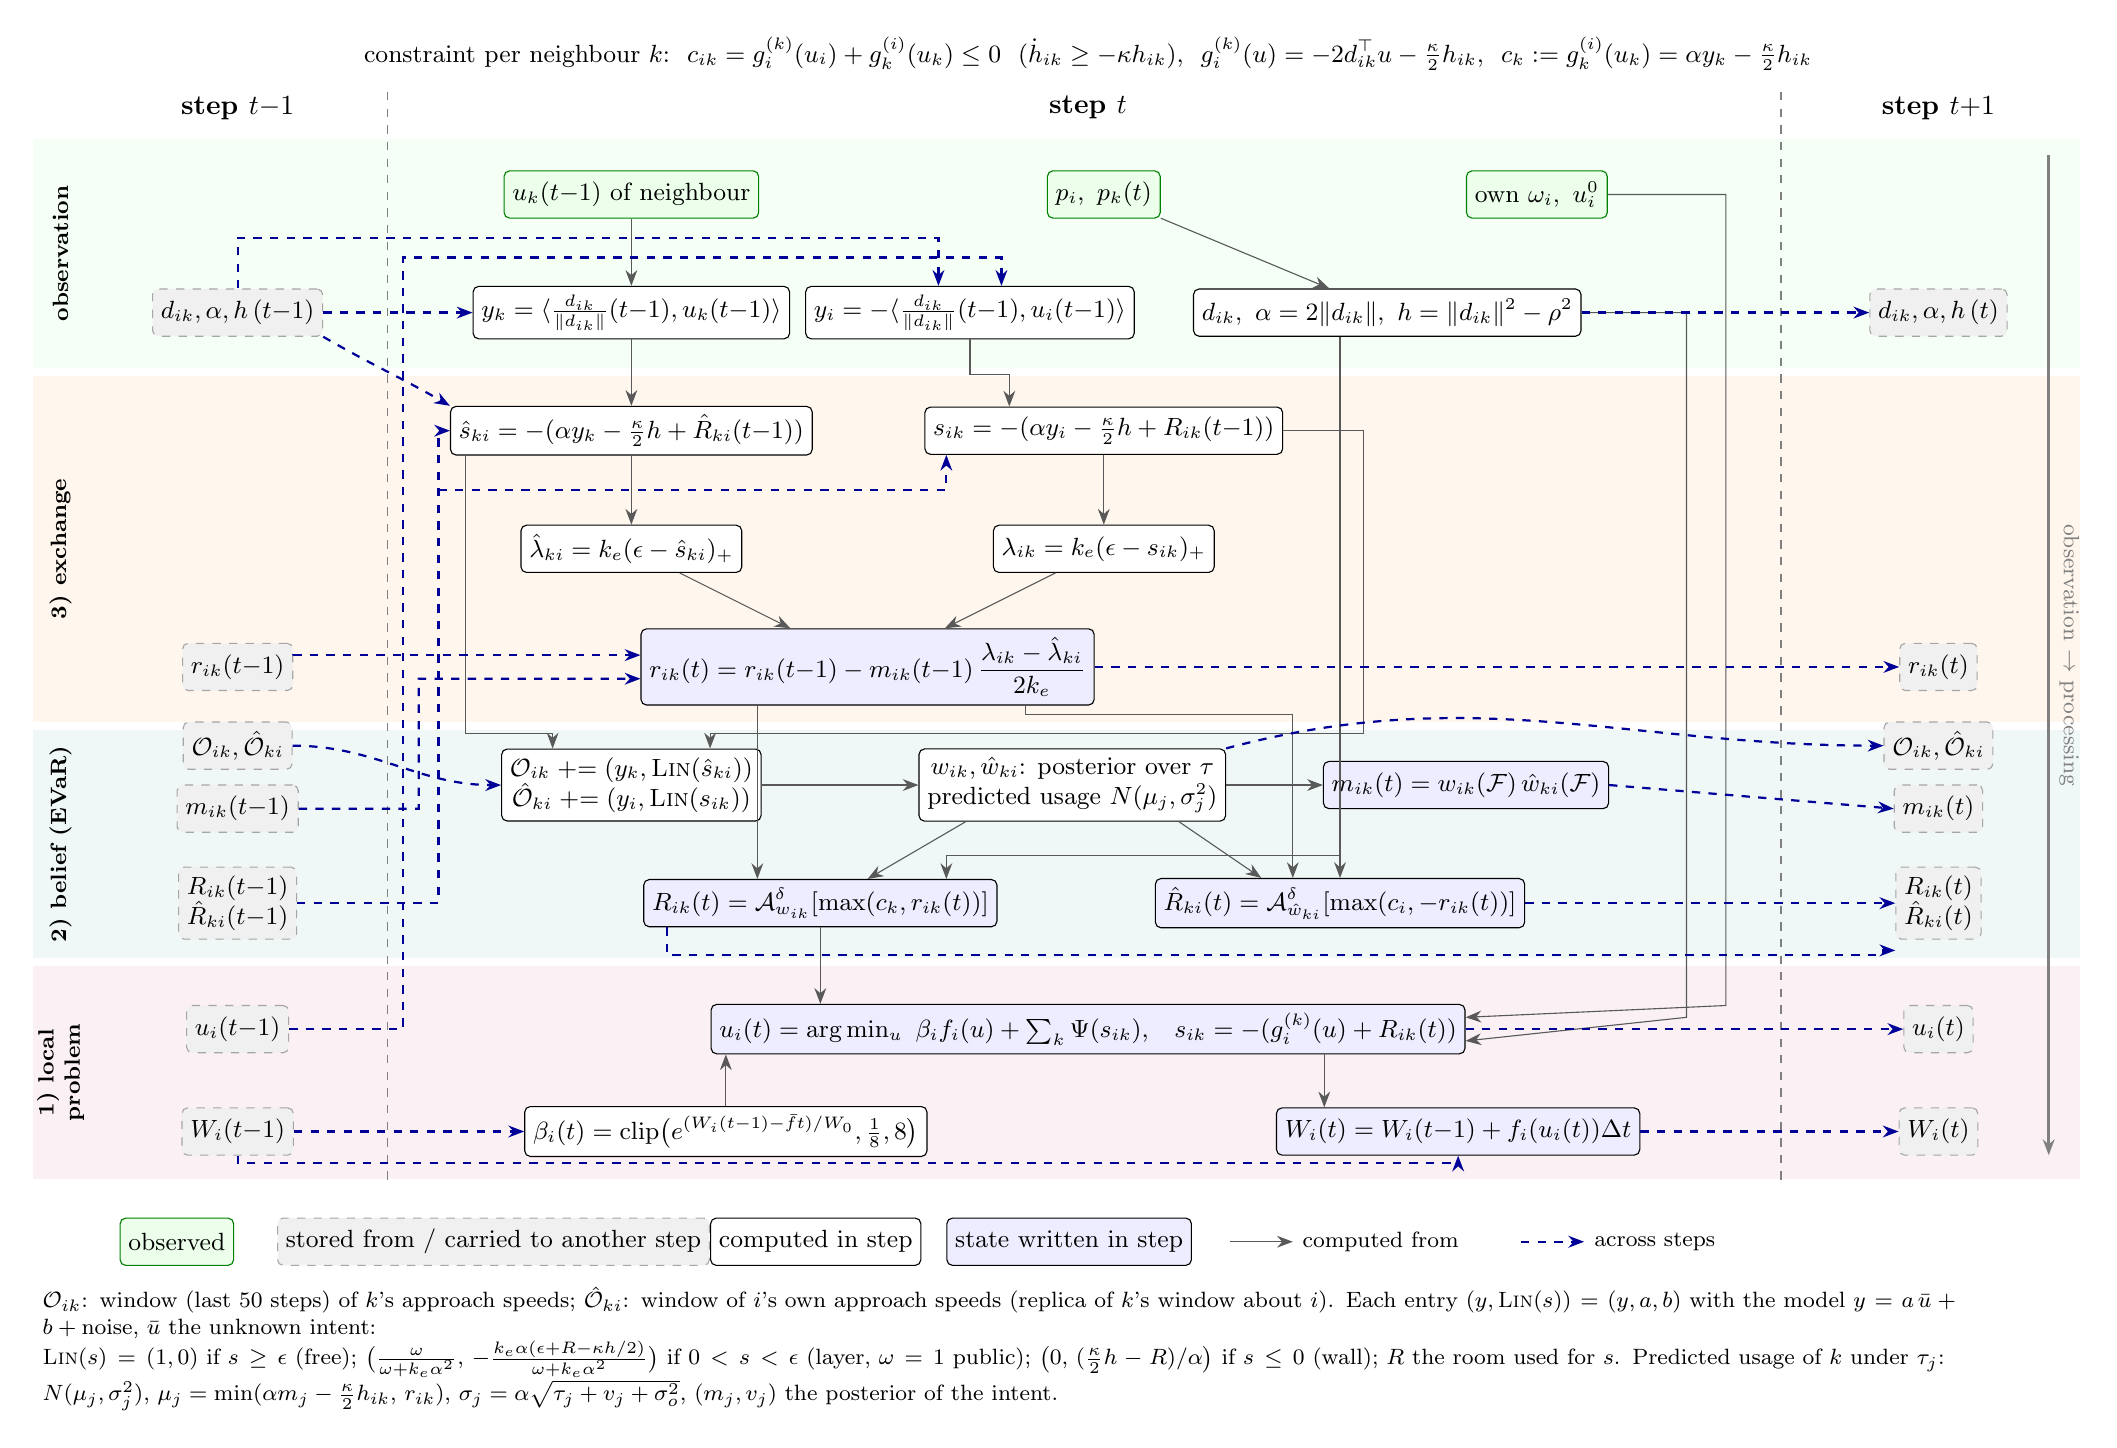
\begin{tikzpicture}[x=1cm,y=1cm,font=\small,>={Stealth[length=2mm]},
  obs/.style={draw=green!50!black,fill=green!8,rounded corners=2pt,inner sep=3pt,minimum height=6mm},
  sto/.style={draw=gray!70,fill=gray!12,dashed,rounded corners=2pt,inner sep=3pt,minimum height=6mm},
  cmp/.style={draw=black,fill=white,rounded corners=2pt,inner sep=3pt,minimum height=6mm},
  st/.style={cmp,fill=blue!7},
  e/.style={->,draw=black!65},
  carry/.style={->,draw=blue!60!black,dashed,thick}]
% rows
\def\yO{0}\def\yD{-1.5}\def\yS{-3}\def\yL{-4.5}\def\yX{-6}\def\yB{-7.5}\def\yR{-9}\def\yQ{-10.6}
% columns
\def\xa{0}\def\xb{21.6}
% ---- row labels and bands ----
\begin{scope}[on background layer]
\fill[green!4] (-2.6,\yO+0.7) rectangle (23.4,\yD-0.7);
\fill[orange!7] (-2.6,\yS+0.7) rectangle (23.4,\yX-0.7);
\fill[teal!6] (-2.6,\yB+0.7) rectangle (23.4,\yR-0.7);
\fill[purple!6] (-2.6,\yQ+0.8) rectangle (23.4,\yQ-1.9);
\draw[gray,dashed] (1.9,1.3)--(1.9,-12.6); \draw[gray,dashed] (19.6,1.3)--(19.6,-12.6);
\end{scope}
\node[font=\bfseries] at (\xa,1.1) {step $t{-}1$};
\node[font=\bfseries] at (10.8,1.1) {step $t$};
\node[font=\small,anchor=south] at (10.8,1.45) {constraint per neighbour $k$:\ \ $c_{ik}=g_i^{(k)}(u_i)+g_k^{(i)}(u_k)\le0$ \ ($\dot h_{ik}\ge-\kappa h_{ik}$),\ \ $g_i^{(k)}(u)=-2d_{ik}^\top u-\tfrac\kappa2h_{ik}$,\ \ $c_k:=g_k^{(i)}(u_k)=\alpha y_k-\tfrac\kappa2h_{ik}$};
\node[font=\bfseries] at (\xb,1.1) {step $t{+}1$};
\node[rotate=90,font=\bfseries\footnotesize] at (-2.25,-0.75) {observation};
\node[rotate=90,font=\bfseries\footnotesize] at (-2.25,-4.5) {3) exchange};
\node[rotate=90,font=\bfseries\footnotesize] at (-2.25,-8.25) {2) belief (EVaR)};
\node[rotate=90,font=\bfseries\footnotesize,align=center] at (-2.25,\yQ-0.55) {1) local\\problem};
\draw[->,very thick,gray] (23.0,0.5)--(23.0,-12.2) node[midway,rotate=-90,above,font=\footnotesize] {observation $\to$ processing};

% ---- step t-1 (stored) ----
\node[sto] (rP) at (\xa,\yX) {$r_{ik}(t{-}1)$};
\node[sto] (dP) at (\xa,\yD) {$d_{ik},\alpha,h\,(t{-}1)$};
\node[sto] (mP) at (\xa,\yB-0.3) {$m_{ik}(t{-}1)$};
\node[sto] (OP) at (\xa,\yB+0.5) {$\mathcal O_{ik},\hat{\mathcal O}_{ki}$};
\node[sto,align=center] (RP) at (\xa,\yR) {$R_{ik}(t{-}1)$\\$\hat R_{ki}(t{-}1)$};
\node[sto] (uP) at (\xa,\yQ) {$u_i(t{-}1)$};
\node[sto] (WP) at (\xa,\yQ-1.3) {$W_i(t{-}1)$};

% ---- step t ----
\node[obs] (uk) at (5,\yO) {$u_k(t{-}1)$ of neighbour};
\node[obs] (pk) at (11,\yO) {$p_i,\ p_k(t)$};
\node[obs] (own) at (16.5,\yO) {own $\omega_i,\ u_i^0$};

\node[cmp] (yk) at (5,\yD) {$y_k=\langle\frac{d_{ik}}{\|d_{ik}\|}(t{-}1),u_k(t{-}1)\rangle$};
\node[cmp] (yi) at (9.3,\yD) {$y_i=-\langle\frac{d_{ik}}{\|d_{ik}\|}(t{-}1),u_i(t{-}1)\rangle$};
\node[cmp] (geo) at (14.6,\yD) {$d_{ik},\ \alpha=2\|d_{ik}\|,\ h=\|d_{ik}\|^2-\rho^2$};

\node[cmp] (sh) at (5,\yS) {$\hat s_{ki}=-(\alpha y_k-\tfrac\kappa2h+\hat R_{ki}(t{-}1))$};
\node[cmp] (si) at (11,\yS) {$s_{ik}=-(\alpha y_i-\tfrac\kappa2h+R_{ik}(t{-}1))$};
\node[cmp] (lh) at (5,\yL) {$\hat\lambda_{ki}=k_e(\epsilon-\hat s_{ki})_+$};
\node[cmp] (li) at (11,\yL) {$\lambda_{ik}=k_e(\epsilon-s_{ik})_+$};
\node[st] (r) at (8,\yX) {$r_{ik}(t)=r_{ik}(t{-}1)-m_{ik}(t{-}1)\,\dfrac{\lambda_{ik}-\hat\lambda_{ki}}{2k_e}$};

\node[cmp,align=center] (O) at (5,\yB) {$\mathcal O_{ik}\mathrel{+}=(y_k,\textsc{Lin}(\hat s_{ki}))$\\$\hat{\mathcal O}_{ki}\mathrel{+}=(y_i,\textsc{Lin}(s_{ik}))$};
\node[cmp,align=center] (post) at (10.6,\yB) {$w_{ik},\hat w_{ki}$: posterior over $\tau$\\ predicted usage $N(\mu_j,\sigma_j^2)$};
\node[st] (m) at (15.6,\yB) {$m_{ik}(t)=w_{ik}(\F)\,\hat w_{ki}(\F)$};
\node[st] (R) at (7.4,\yR) {$R_{ik}(t)=\A^\delta_{w_{ik}}[\max(c_k,r_{ik}(t))]$};
\node[st] (Rh) at (14.0,\yR) {$\hat R_{ki}(t)=\A^\delta_{\hat w_{ki}}[\max(c_i,-r_{ik}(t))]$};

\node[st,align=center] (qp) at (10.8,\yQ) {$u_i(t)=\arg\min_u\ \beta_if_i(u)+\sum_k\Psi(s_{ik})$,\quad $s_{ik}=-(g_i^{(k)}(u)+R_{ik}(t))$};
\node[cmp] (bt) at (6.2,\yQ-1.3) {$\beta_i(t)=\mathrm{clip}\big(e^{(W_i(t-1)-\bar f t)/W_0},\tfrac18,8\big)$};
\node[st] (Wt) at (15.5,\yQ-1.3) {$W_i(t)=W_i(t{-}1)+f_i(u_i(t))\Delta t$};

% ---- step t+1 (carried) ----
\node[sto] (rN) at (\xb,\yX) {$r_{ik}(t)$};
\node[sto] (dN) at (\xb,\yD) {$d_{ik},\alpha,h\,(t)$};
\node[sto] (mN) at (\xb,\yB-0.3) {$m_{ik}(t)$};
\node[sto] (ON) at (\xb,\yB+0.5) {$\mathcal O_{ik},\hat{\mathcal O}_{ki}$};
\node[sto,align=center] (RN) at (\xb,\yR) {$R_{ik}(t)$\\$\hat R_{ki}(t)$};
\node[sto] (uN) at (\xb,\yQ) {$u_i(t)$};
\node[sto] (WN) at (\xb,\yQ-1.3) {$W_i(t)$};

% ---- arrows within step t ----
\draw[e] (uk)--(yk); \draw[e] (pk)--(geo); \draw[e] (geo.south -| Rh.north)--(Rh.north); \draw[e] (Rh.north |- 0,-8.4) -| ([xshift=16mm]R.north);
\draw[e] (yk)--(sh); \draw[e] (yi.south)--++(0,-0.45)-|([xshift=-12mm]si.north);

\draw[e] (sh)--(lh); \draw[e] (si)--(li);
\draw[e] (lh)--(r); \draw[e] (li)--(r);
\draw[e] ([xshift=2mm]sh.south west)--([xshift=2mm]sh.south west |- 0,-6.85)-|([xshift=-10mm]O.north);
\draw[e] (si.east)-|(14.3,-6.85)-|([xshift=10mm]O.north);
\draw[e] (O)--(post); \draw[e] (post)--(m);
\draw[e] (post.south west)++(0.6,0)--([xshift=6mm]R.north); \draw[e] (post.south east)++(-0.6,0)--([xshift=-10mm]Rh.north);
\draw[e] ([xshift=-14mm]r.south)--([xshift=-14mm]r.south |- R.north); \draw[e] ([xshift=20mm]r.south)--([xshift=20mm]r.south |- 0,-6.6)-|([xshift=-6mm]Rh.north);
\draw[e] (R.south)--(R.south |- qp.north);
\draw[e] (geo.east)-|(18.4,-10.45)--([yshift=-1.5mm]qp.east);
\draw[e] (own.east)-|(18.9,-10.3)--([yshift=1.5mm]qp.east);

% ---- arrows from t-1 ----
\draw[carry] (dP.east)--(yk.west);
\draw[carry] (dP.north)|-(3.0,-0.55)-|([xshift=-4mm]yi.north);
\draw[carry] (dP.south east) to[out=-30,in=150] (sh.north west);
\draw[carry] (rP)--([yshift=1.5mm]r.west -| rP.east) -- ([yshift=1.5mm]r.west);
\draw[carry] (mP.east)-|(2.3,-6.15)--([yshift=-1.5mm]r.west);
\draw[carry] (OP.east) to[out=0,in=180] (O.west);
\draw[carry] (RP.east)-|(2.55,\yS)--(sh.west);
\draw[carry] (2.55,-3.75)-|([xshift=-20mm]si.south);
\draw[carry] (uP.east)-|(2.1,-0.8)-|([xshift=4mm]yi.north);
\draw[carry] (WP.east)--(bt.west);
\draw[e] (bt.north)--(bt.north |- qp.south);
\draw[e] ([xshift=30mm]qp.south)--([xshift=30mm]qp.south |- Wt.north);
\draw[carry] (Wt.east)--(WN.west);
\draw[carry] (WP.south)--(WP.south |- 0,-12.3)-|(Wt.south);

% ---- arrows to t+1 ----
\draw[carry] (r.east) -- (rN.west);
\draw[carry] (geo.east)--(dN.west);
\draw[carry] (m.east)--(mN.west);
\draw[carry] (post.north east) to[out=15,in=180] (ON.west);
\draw[carry] (Rh.east)--(RN.west);
\draw[carry] (R.south west)++(0.3,0)--++(0,-0.35)-|(20.9,-9.6)--(20.9,-9.6 -| RN.west);
\draw[carry] (qp.east)--(uN.west);

% legend
\node[obs,anchor=west] (L1) at (-1.5,-13.3) {observed};
\node[sto,anchor=west] (L2) at (0.5,-13.3) {stored from / carried to another step};
\node[cmp,anchor=west] (L3) at (6.0,-13.3) {computed in step};
\node[st,anchor=west] (L4) at (9.0,-13.3) {state written in step};
\draw[e] (12.6,-13.3)--(13.4,-13.3) node[right,font=\footnotesize] {computed from};
\draw[carry] (16.3,-13.3)--(17.1,-13.3) node[right,font=\footnotesize] {across steps};
\node[anchor=north west,font=\footnotesize,align=left,text width=24.5cm] at (-2.6,-13.75) {$\mathcal O_{ik}$: window (last 50 steps) of $k$'s approach speeds; $\hat{\mathcal O}_{ki}$: window of $i$'s own approach speeds (replica of $k$'s window about $i$). Each entry $(y,\textsc{Lin}(s))=(y,a,b)$ with the model $y=a\,\bar u+b+\text{noise}$, $\bar u$ the unknown intent:\\ $\textsc{Lin}(s)=(1,0)$ if $s\ge\epsilon$ (free); $\big(\frac{\omega}{\omega+k_e\alpha^2},\,-\frac{k_e\alpha(\epsilon+R-\kappa h/2)}{\omega+k_e\alpha^2}\big)$ if $0<s<\epsilon$ (layer, $\omega=1$ public); $\big(0,\,(\tfrac\kappa2h-R)/\alpha\big)$ if $s\le0$ (wall); $R$ the room used for $s$. Predicted usage of $k$ under $\tau_j$: $N(\mu_j,\sigma_j^2)$, $\mu_j=\min(\alpha m_j-\tfrac\kappa2h_{ik},\,r_{ik})$, $\sigma_j=\alpha\sqrt{\tau_j+v_j+\sigma_o^2}$, $(m_j,v_j)$ the posterior of the intent.};
\end{tikzpicture}
\end{document}
